
\documentclass[a4j,10pt]{jsarticle}
\usepackage{layout,url,resume}
\usepackage[dvipdfmx]{graphicx}
\pagestyle{empty}

\begin{document}
%\layout

\title{[TERM]RGBカメラによる自律飛行経路探索手法の提案}

% 和文著者名
\author{
    著者その1 {井手田 悠希} \thanks{慶應義塾大学 環境情報学部 武田圭史研究室}
}

% 和文概要
\begin{abstract}
現時点で安価で広く流通している上に小型のものも多く存在するRGBカメラによる自律飛行経路探索手法を提案する.
現在自律飛行で多く使用されるLIDARなどのセンサーは他の超音波やRGBカメラに比べて高価であり,またサイズも広く流通しているものは大きい物が多い.
そこで,本研究では比較的安価で手に入り小型の物も多く流通しているRGBカメラを利用した自律飛行制御を目指す.

本研究では障害物が多く存在する屋内でのランダムウォークを第1段階の目標とし.また,これらに加えて本研究では人物追従や他のドローンの追従,追従しているドローンによる被追従ドローンの制御を目標最終的な到達目標としている.
将来的には郡飛行時のドローンの制御や観測,屋内の倉庫など複数のドローンが様々な方向に飛び交うような環境においての衝突を避けるような技術として応用をしていきたい.

\end{abstract}

\maketitle
\thispagestyle{empty}

\section{はじめに}
本研究を行うに至った動機として現在のドローンでの物資輸送への違和感である.
ドローンを映像で制御する今後の展望として,ドローンの第3者視点映像による高精度制御がある.
これは物資輸送を行う際に,現時点では運ぶ物資に合わせてそれぞれに合った積載量のドローンを用意しなければならない.
しかしこの状況は産業利用や日常利用などで様々な大きさ重さの物資を運ぶことが想定される環境においては管理コストが単一機種を複数所持するのに対して大きくなると考えられる.
そこで,ドローン所持における管理コストを下げる為に,大型の物資は複数の中型機で輸送し,それ以外は1機で輸送したい.

これらを実現する上で複数ドローンが密集した状態での高精度制御が要求される.その前段階の技術として,ドローンをRGBカメラの映像によって制御することを実現したい.

\section{背景}
2010年頃からParrot社による家庭用ドローンの発売などもあり,これ以降ドローンの認知と研究開発は加速している.
付随して,自律飛行に関しても研究が盛んに行われているが,現在行われている自律飛行ではLIDARなど他のセンサーと比較して高価なものを使用している例が多い.

また広く流通しているものは大きいものばかりである.これらの問題はドローンでの活用がさらに進めばセンサー自体の開発も進み解決するだろう.しかし,LIDAR等のセンサー以外を主とした飛行経路探索手法を模索することは今後の自律飛行の精度向上に貢献すると考え,本研究を実施するに至った.


\section{研究目的}
本研究の目的はドローンの制御精度向上であり,本手法を単体で飛行経路選択をする以外にも,他のLIDARなどのセンサーも合わせて使用するような制御系における,制御の一助となるような使用を想定している.
また,RGBカメラの特性上雨天時や夜間などは著しく精度が低下する事が予測される為,基本的には屋内や,明るさがある程度確保できる条件下での使用を想定している.
その中で,本手法で用いる物体検知アルゴリズムではRGBカメラによる映像を使用する為,LIDAR等の他センサを利用するよりも安価に視野画内にある物体の意味を理解することができる.その点でLIDARなどの手法に比べて物体の特性なども考慮した判断をすることができる点が他の手法との異なる点である.
最終的には目の前にある物体が設置物なのか,移動物体なのか等を判断した上での飛行経路の選択をする事で屋内での飛行などでもより急な制御をする事なく事前に停止したり,回避行動をとれるようになると考えられる.
現在路面を走る車両には信号機がある為スムーズに飛行が行えるが,飛行物体に対する信号機は無い.しかし,今後様々な用途で飛び交うドローンが他のドローンと遭遇する機会が発生することは容易に想像でき,遭遇した際の事故を避ける技術が求められる.
そこで,本研究ではドローンに積載されたRGBカメラの映像からの情報を元に機体の飛行経路を選択するアルゴリズムを提案する.

\section{関連研究}
基本的にドローンが自律飛行を行う際に必要とされる処理がいくつかある.そのうちの2つが自己位置推定と姿勢推定である.
自己位置推定とは,ドローンが飛行している空間の中で自分がどの位置にいるのかを認識する事である.姿勢推定とは自分が水平方向に対してどの程度傾いているのか,鉛直方向に対してどの程度回転しているかを認識することある.

本研究では主に自己位置推定を行い,その上で得られる周囲の情報を元にどのような飛行経路を取るかについての処理系について論を進めていく.

関連研究として強く影響を受けているものが Nanomap\cite{Nanomap}である.
Nanomapにおいては2D-LIDARを用いた飛行経路探索手法が取られており,取得した点群データを過去数フレーム分を記憶しておき,過去の数フレーム分のデータと現在のフレームとの点群の変量によっておおよその障害物の位置を認識している.こちらの手法では,物体を正確に捉えることは放棄し,不確実な部分を物体の存在している可能性のある範囲として捉えている.視野にある物体のある可能性も含めて1番物体が少ない方向を飛行経路として選定し,飛行している.

他に,ドローンに限らずロボット工学全般で利用されてきたOctomap\cite{Octomap}がある.
こちらもNanomapと同様にLIDARを用いて周辺の環境情報を扱うものであるが,こちらはLIDARを用いて実際に周囲を点群からモデリングして周辺状況を把握する.

Octomapではモデリングする際に近い点群同士を同じ物体としてまとめ1つのブロックにするということを繰り返し,樹構造的に物体を生成する為,生成後のデータは繰り返す回数等のパラメータによっては小さく圧縮することもできる.
しかし,実際に点群からモデルを生成するとなるとその計算量は非常に多く,高性能な小型コンピュータが現れている現在においても処理負荷が大きく,特にドローンにおいては積載量に制限がかかりやすい為扱いにくいものとなっている.

また,これらのようにLIDARを使用せず,CMOSセンサーのみで自律飛行を行なっている例もある.

実用性を備えた手のひらサイズ・完全オンボード処理 UAV のための 3 次元自己位置推定手法の提案と全自動飛行の実現\cite{SfMDrone}では自己位置推定で使用するセンサーはCMOSセンサーを利用した自律飛行を実現している.
CMOSセンサーからの映像をFPGAにストリームしてFAST\cite{FAST}による特徴点抽出処理を行い,その結果をBrief\cite{Brief}を用いて表現し,MCUに流し込み処理している.この研究での目的は外部処理系に依存せず,ドローン上で全て完結する自律飛行可能な小型ドローンの開発で,限定条件下(新聞紙を敷き詰めた床面)の上で飛行させ,特徴点を十分に検出できるようにした上で,飛行させ想定通りの飛行を実現している.


\section{提案手法}
本手法では2つの部分に分かれて処理をする.まず1つ目は飛行経路を探索する処理系.もう1つが周囲の環境を認識して動く可能性の高い物体なのか,そうでない物体なのかを分類し,動く可能性の高い物体に対してはより排他的空域を広く取り,そこに侵入しないように飛行経路を選択する.
ここでいう排他的空域は動く可能性が低いものに対してもそうでない物に対しても全ての検出物に対して設定されている.

\begin{figure}[htbp]
  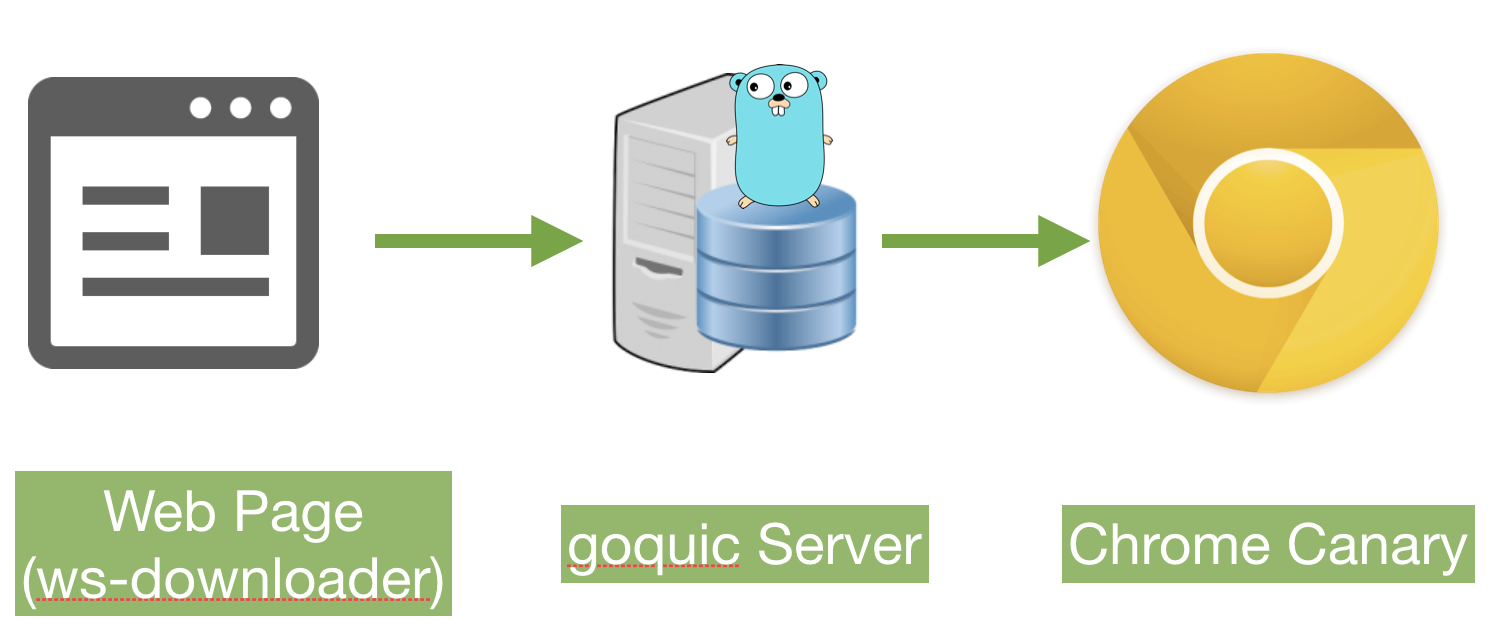
\includegraphics[width=7cm]{figure1.png}
  \caption{動く可能性の低い物体}
\end{figure}
\begin{figure}[htbp]
  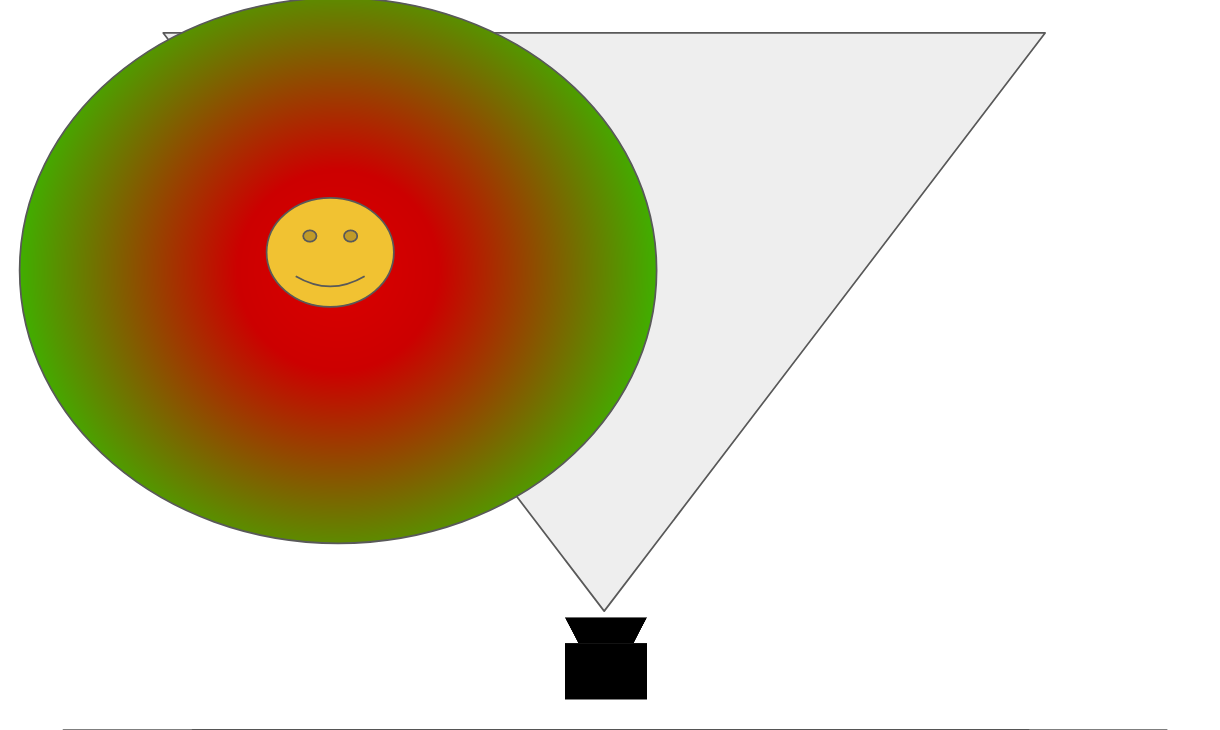
\includegraphics[width=7cm]{figure2.png}
  \caption{動く可能性の高い物体}
\end{figure}

まず,1つ目の飛行経路探索を行う処理系に関しては以下の条件を判断軸にして経路選択,飛行を行うものとする.

\begin{enumerate}
\item 視野の中に移る検出された物体の中で画面占有率の高いものをより重要度が高いものとして設定する.
\item 検出される物体が一番少ない何もない所を一番安全な方向として設定する.
\item 何も検出されなくなった場合,大きな平面に直面したとして一時停止する.
\end{enumerate}

次に2つ目の検出した物体の属性を判定する部分であるが,こちらは検出時にラベルが得られるのでそのラベルをキーとして辞書データから検出する事とする.
また,おおよその移動速度も物によって推測でき,辞書データの中に含める事で,排他的空域をどこまで広げるかを設定する.
動くことが想定される物体よりも高い位置で飛ぶ際もその直上は落下可能性を拭いきれないので飛行禁止空域として設定する.

実際に使用する技術としては以下のものを使用する.
\begin{itemize}
\item Tello
\item MacBookPro 2016Model
\item Yolo v3
\item Golang (後々Python3に変更する可能性も)
\item Gobot(Golangのロボティクス向けフレームワーク)
\end{itemize}

\section{評価}
空き教室でランダムウォークさせ,何秒間無衝突で飛行できるかを評価する.
1分以上問題なく飛行できるようであれば研究室に場所を移し,再度同様の実験を行う.
それでも問題ないようであれば屋外に場所を移し,木が複数生えている所で同様の実験を行う.

\section{考察}


\begin{thebibliography}{99}
%\bibitem{a}
\bibitem{Nanomap}
\texttt{Peter R. Florence1, John Carter1, Jake Ware1, Russ Tedrake1, NanoMap: Fast, Uncertainty-Aware Proximity Queries with Lazy Search over Local 3D Data}

\bibitem{Octomap}
\texttt{A. Hornung, K. M. Wurm, M. Bennewitz, C. Stachniss, and W. Burgard, “Octomap: An efficient probabilistic 3d mapping framework based on octrees,” Auton. Robots, vol. 34, no. 3, pp. 189–206, Apr. 2013. [Online]. Available: http://dx.doi.org/10.1007/ s10514- 012- 9321- 0}

\bibitem{Voxblox}
\texttt{H. Oleynikova, Z. Taylor, M. Fehr, J. Nieto, and R. Siegwart, “Voxblox: Building 3d signed distance fields for planning,” arXiv preprint arXiv:1611.03631, 2016.}

\bibitem{SfMDrone}
\texttt{此村 領, 堀 浩1, 実用性を備えた手のひらサイズ・完全オンボード処理 UAV のための 3 次元自己位置推定手法の提案と全自動飛行の実現, 東京大学工学系研究科航空宇宙工学専攻}

\bibitem{FAST}
\texttt{E. Rosten, R. Porter, and T. Drummond. “Faster and better: A machine learning approach to corner detection.” IEEE Trans. Pattern Analysis and Machine Intelligence, 32:105-119, 2010.}

\bibitem{Brief}
\texttt{M. Calonder, V. Lepetit, C. Strecha, and P. Fua. “Brief: Binary robust independent elementary features.” In European Conference on Computer Vi- sion, 2010.}

\end{thebibliography}

\end{document}
% end of file
